\documentclass{article}
\usepackage{style}
\usepackage[utf8]{inputenc}
\usepackage{placeins}
\usepackage{booktabs} 
\usepackage{longtable}
\usepackage[title]{appendix}
\usepackage{amssymb}

\graphicspath{{media/}}

\title[Primality Testing]{Probabilistic Primality Testing and Analysis of Probabilistic AKS}
\author[Emilie Ma]{%
Emilie Ma\\%
University of British Columbia\\%
\texttt{kewbish@gmail.com}%
}
\date{\today}
\mentor{Pressiana Marinova\\%
Ocado Technology Sofia\\%
\texttt{pressiana.marinova@gmail.com}%
}

\begin{document}
\maketitle
\newpage
\begin{abstract}
This paper aims to analyze the Fermat, the Euler (Solovay-Strassen), and the Miller-Rabin primality tests, three well-known probabilistic algorithms based on Fermat's little theorem. The Agarwal-Kayal-Saxena test, the first polynomial time deterministic primality test developed, is also discussed, as well as a proposal for a new probabilistic adaptation. This probabilistic AKS was found to deliver significant running time decreases, at the expense of eliminating determinism and passing a considerable amount of pseudoprimes.
\end{abstract}

\section{Introduction}
Prime numbers, or numbers with no factors other than 1 and itself, are of crucial importance in cryptography and cybersecurity. Many encryption algorithms, such as the frequently used Rivest-Shamir-Adleman (RSA) cryptosystem, rely on the `trapdoor' nature of prime numbers: while multiplying prime numbers is trivial, finding the factors of a composite number is computationally expensive. Since cryptography is so widely applied in modern systems, generating prime numbers for use in encryption cryptosystems is a major field of research in computer science and mathematics.

To generate a prime number, many algorithms first generate a random number $n$. This number $n$ is then passed through a primality test, an algorithm designed to identify if a number is prime or not. A variety of primality tests may be used, including the Fermat, Euler or Solovay-Strassen, Miller-Rabin, and Agarwal-Kayal-Saxena (AKS) tests.

These tests, except the AKS test, are \emph{probabilistic}. A probabilistic test is an algorithm that utilizes some form of randomness in its design; for example, random bases may be selected from a range of possibilities to be tested. In contrast, a deterministic algorithm, when given an input, will always return the same output. Minimizing the running time of primality tests is desired to increase the efficiency of generating random primes, so probabilistic tests are often used due to their shorter average running time and increased practicality. However, probabilistic tests have a small probability of wrongly designating a composite number as prime. This is avoided with deterministic primality tests, such as the AKS test, but issues with impractical running times arise.

The AKS test is notable for being the first polynomial time deterministic primality test. Polynomial time refers to a concept of Big-O theory, the notation that describes the upper bound of a function when its input tends towards infinity. In Big-O notation, polynomial time, or a function of form $O(n^x)$ is preferred to exponential time, or a function of form $O(x^n)$ for some input size $n$ and value $x$, as $x^n$ will grow faster than $n^x$ as $n$ increases. In other words, $n^x$ algorithms are more efficient than $x^n$ ones in worst-case scenarios. 

However, even though AKS is bounded by polynomial time, it remains impractical and incredibly slow compared to probabilistic tests. As Brent showed in a 2010 comparison with the Miller-Rabin and other probabilistic primality tests, it was found that where 100 trials of Miller-Rabin took 0.3 seconds to process, AKS would take an estimated 37 weeks to run one trial on the same number (equivalent, as AKS is deterministic and only requires one run to determine the output) \cite{brent_primality_2010}. These times are unfeasibly large for applied usage, so research into optimizing and discovering probabilistic tests remains relevant.

As an alternative to AKS, this paper proposes a probabilistic version of AKS, inspired by the technique used by the Fermat, Euler (Solovay-Strassen), and Miller-Rabin tests in choosing a range of random numbers to test against certain congruences and theorems. This probabilistic AKS was analyzed for average number of pseudoprimes returned given a certain number $k$ of equations to test, as well as for decreases in elapsed wall-time and increases in runtime efficiency. It was found that probabilistic AKS was significantly faster than deterministic AKS, though passed high numbers of pseudoprimes at low numbers of equations checked.

\section{Background Number Theory}

Many probabilistic primality tests rely on number theory proofs and modular arithmetic to test for primality. The Fermat, Euler (Solovay-Strassen), Miller-Rabin, and AKS tests, as well as their background theory, are discussed below.

Note that all $\log{n}$ in this paper are assumed to be taken as $\log_{2}{n}$ unless otherwise marked.

\subsection{Fermat Primality Test}
The Fermat Primality Test is a probabilistic primality test based on Fermat's little theorem.
Fermat's little theorem, developed by Fermat in 1640, states that for any integer $a$ and any prime $p$, the following holds:
\[
    a^p \equiv a \pmod{p} 
\]
If $a$ is not divisible by, or \emph{coprime} to, p, the following is equivalent:
\[
    a^{(p - 1)} \equiv 1 \pmod{p} 
\]

\begin{proof}
Note that $p \vert a$ is equivalent to $a \equiv 0 \pmod{p}$.
Assume $gcd(a, n) = 1$; in other words, $a$ and $n$ are coprime.
Consider $S = \{a, 2a, \ldots{}, (p - 1) \times a\}$.
Suppose $ra$ and $sa$ in the set are equal $\pmod{p}$, so $r \equiv s \pmod{p}$ because $p \nmid a$.
Therefore, the $p - 1$ multiples of $a$ in $S$ are uniquely distinct, and must be congruent to ${1, 2, \ldots{}, (p - 1)}$ in some order.
Multiply these congruences like so:
    \[a \times 2a \times \ldots{} \times (p - 1)a \equiv 1 \times 2 \times 3 \times \ldots{} (p - 1) \pmod{p}\]
This gives:
    \[a^{(p - 1)} \times (p - 1)! \equiv (p - 1)! \pmod{p}\]
$p$ does not divide $(p - 1)!$, so divide by $(p - 1)!$ on each side for:
    \[a^{(p - 1)} \equiv 1 \pmod{p}\]
To arrive at the alternate form of Fermat's Little Theorem, multiply both sides by $a$:
    \[a^p \equiv a \pmod{p}\]
\end{proof}

Knowing that $a^{(n - 1)} \equiv 1 \pmod{n}$ holds if $n$ is prime, Fermat's primality test chooses $k$ random integers $a$ coprime to $n$ to test if all $a$ are congruent to 1. Because this holds trivially for $a \equiv 1 \pmod{n}$ and if $n$ is odd and $a \equiv -1 \pmod{n}$, $a$ is conventionally chosen such that $1 < a < n - 1$. Higher values of $k$ provide a higher probability that the number is prime.

If $n$ passes these $k$ base tests, it is known as a Fermat probable prime. However, not all numbers that pass the Fermat primality test are prime - composite numbers $n$ that pass the test are known as Fermat pseudoprimes. There are infinitely many Fermat pseudoprimes, and several known forms of composite numbers that pass the test. For example, Carmichael numbers, composite numbers that satisfy the relation $b^{(n-1)} \equiv 1 \pmod{n}$ for all integers $b$ coprime to $n$, all pass Fermat's primality test.

\subsection{Euler (Solovay-Strassen) Test} % https://artofproblemsolving.com/wiki/index.php/Euler%27s_Totient_Theorem
The Solovay-Strassen Test is another probabilistic test, utilizing properties of Euler's theorem \cite{solovay_fast_1977}. Proposed by Euler in 1763, Euler's theorem is a generalization of Fermat's little theorem, stating that if $a$ and $p$ are coprime, then the following holds:
\[
    a^{\phi(n)} \equiv 1 \pmod{n}
\]
The function $\phi(n)$ is Euler's totient function. The totient of some number $n$ is the number of positive integers $l$ in the range $1 \leq l \leq n$ where l is coprime to n.

\begin{proof}
    Consider $S = \{1 \leq l \leq n | gcd(l, n) = 1\} = \{l_1, l_2, l_3, \ldots{}, l_{\phi(n)}\}$.
    Create a set $aS = \{al_1, al_2, al_3, \ldots{}, al_{\phi(n)}\}$. \\
    All elements of $aS$ are relatively prime to $n$, so if all elements of $aS$ are distinct, $aS = S$. All elements of $aS$ are distinct, as all elements of $S$ are distinct. Therefore, each element of $aS \equiv S \pmod{n}$.
    Therefore:
    \[
        l_1 \times l_2 \times l_3 \times \ldots{} \times l_{\phi(n)} \equiv al_1 \times al_2 \times al_3 \times \ldots{} \times al_{\phi(n)} \pmod{n}
    \]
    As $l_1 \times l_2 \times l_3 \times \ldots{} \times l_{\phi(n)}$ is relatively prime to $n$, reducing this gives:
    \[
        a^{\phi(n)} \times l_1 \times l_2 \times l_3 \times \ldots{} \times l_{\phi(n)} \equiv l_1 \times l_2 \times l_3 \times \ldots{} \times l_{\phi(n)} \pmod{n}
    \]
    Therefore, $a^{\phi(n)} \equiv 1 \pmod{n}$.
\end{proof}

Fermat's little theorem is considered a special case of Euler's theorem, because if $n$ is prime, $\phi(n) = n - 1$.

Given that $a^{\phi(n)} \equiv 1 \pmod{n}$, then:
\[
    a^{\phi(n) / 2} \equiv \begin{cases}
\;\;\,1\pmod{n}& \text{ when there exists }x \text{ such that }a\equiv x^2 \pmod{n}\\
     -1\pmod{n}& \text{ when there is no such integer.}
\end{cases}
\]

The conditions above form the criteria for the Legendre symbol of $a$ and $n$. The Legendre symbol $\left(\frac{a}{n}\right)$ is defined like so:
\[
    \left(\frac{a}{n}\right) \begin{cases}
        0 & \text{ when $a \equiv 0 \pmod{n}$} \\
        -1& \text{ when $a \not\equiv 0 \pmod{n}$ and there exists $x: a \equiv x^2 \pmod{n}$} \\
     -1& \text{ when $a \not\equiv 0 \pmod{n}$ and there is no such integer $x$.}
\end{cases}
\]

The Jacobi symbol is the generalization of the Legendre symbol to any odd integer $n$, and is used in the Solovay-Strassen primality test. It is defined as the product of the Legendre symbols of $n$'s prime factors, such that:
\[
    \left(\frac{a}{n}\right) = \left(\frac{a}{p_1}\right)^{\alpha_{1}} \times \left(\frac{a}{p_2}\right)^{\alpha_{2}} \times \ldots{} \times \left(\frac{a}{p_k}\right)^{\alpha_{k}}
\]
for $n = p_1^{\alpha_{1}} \times p_2^{\alpha_{2}} \times \ldots{} \times p_k^{\alpha_{k}}$.

As with Fermat's primality test, $k$ random bases $a$ are tested. If $a^{(n - 1) / 2} \equiv (\frac{a}{n}) \pmod{n}$ holds for all $k$ bases, then $n$ is an Euler (or Solovay-Strassen) probable prime.

Similar to Fermat's primality test, the Solovay-Strassen test may pass composite numbers as primes. These are then known as Euler (sometimes Euler-Jacobi) pseudoprimes or liars. All Euler pseudoprimes are also Fermat pseudoprimes. 

\subsection{Miller-Rabin Primality Test}
A third probabilistic primality test, the Miller-Rabin primality test was developed by Miller in 1975 \cite{miller_riemanns_1975}, and subsequently modified by Rabin in 1980 \cite{rabin_probabilistic_1980}. The test relies on two congruence relations that hold when $n$ is an odd prime and rewritten as $2^s \times d + 1$, and $a$ is a base such that $0 < a < n$:
\begin{gather*}
    a^d \equiv 1 \pmod{n} \\
    a^{(2^r \times d)} \equiv -1 \text{ for some $r$ such that $0 \leq r < s$}
\end{gather*}

Because $n$ is written as $2^s \times d + 1$, $n - 1 = 2^s \times d$. Therefore, if $a^d \equiv \pm 1 \pmod{n}$, then $n$ is a strong probable prime.

\begin{proof}
    Given that:
    \[
        a^{(n - 1)} \equiv (a^d)^{2^s} \equiv 1 \pmod{n}
    \]
    for all prime $n$, and because there are no square roots of 1 other than $\pm 1$, the repeated squaring with $2^s$ does not affect the congruence.
\end{proof}

Otherwise, $a^d \pmod{n}$ is squared, for $a^2d$. If $a^{2d} \equiv 1 \pmod{n}$, n is composite, because there are different square roots of $a^{2d} \pmod{n}$ other than $\pm 1$. If $a^{2d} \equiv -1 \pmod{n}$, then $n$ is a probable prime for similar reasons as above.

These checks are repeated until $a^{(2^{(s - 1)} \times d)}$ has been reached. If it is $\pm 1$, the result is known by the tests above; however, if not, $n$ is composite, by Fermat's little theorem.

\subsection{Agarwal-Kayal-Saxena (AKS) Primality Test}
\label{theory:aks}
By contrast, the AKS primality test is a deterministic primality test first proprosed by Agarwal, Kayal, and Saxena in 2002. It is the first primality test to deterministically verify primality in polynomial time for all number inputs, with a time complexity bound of $\widetilde{O}(\log{(n)}^{15/2})$.

The test is based on the theorem that an integer $n \geq 2$ and an integer $a$ coprime to $n$, $n$ is prime if and only if the below holds within the polynomial ring $\mathbb{Z}[x]$, or the ring of polynomials with degree at most $n$ over $\mathbb{Z}$.
\[
    (X + a)^n \equiv X^n + a \pmod{n}
\]

\begin{proof} % http://www.cs.tau.ac.il/~amnon/Classes/2019-Derandomization/Lectures/Lecture7-AKS-All.pdf
    This is a generalization of Fermat's little theorem over polynomials, proven with the binomial identity.
    \[
        (x + a)^n = \sum_{i=0}^{n} \binom{n}{i} x^i a^{n - i} \text{ where } \binom{n}{0} = \binom{n}{n} = 1
    \]
    If $n$ is prime, then:
    \[
        \binom{n}{i} = \frac{n \times (n - 1) \times \ldots{} \times (n - i + 1)}{i!}
    \]
    for all $i > 1$. When taken $\bmod{n}$, $n$ divides the numerator once; therefore, $\binom{n}{i} \equiv 0 \pmod{n}$. $a$ does not necessarily need to be coprime with $n$.
    If $n$ is not prime, and $a$ is coprime with $n$, then $n$ has a prime factor of form $p^k$. $p^k$ will divide $n$, but $p^{k - 1}$ will not. Given the monomial with a coefficient of:
    \[
        \binom{n}{i} = \frac{n \times (n - 1) \times \ldots{} \times (n - p + 1)}{p!}
    \]
    $p^k$ divides $n$, but not $(n - 1) \ldots{} (n - p + 1)$. Therefore, $p^k \vert n (n - 1) \ldots{} (n - p + 1)$ but $p^{k + 1} \nmid n (n - 1) \ldots{} (n - p + 1)$. $p$ also divdes $p$, but not $1 \ldots p$, so $p \vert p!$ but $p^2 \nmid p!$. This gives $p^{k - 1} \vert \binom{n}{p}$ and $p^k \nmid \binom{n}{p}$. As $p^k$ is a factor of $n$, $n \nmid \binom{n}{p}$, and $x^p$ does not vanish.
\end{proof}

The steps of the algorithm are as follows:
\begin{enumerate}
    \item The test begins by ensuring $n$ is not a perfect power, or a number of form $a^k$ for some $a$ and $k$. If it is, the number is composite.
    \item Next, the algorithm finds the smallest $r$ such that $\textrm{ord}_r(n) > {\log{n}}^2$ and $r$ is coprime to $n$.
    \item The algorithm then checks for all $2 \leq a \leq \min{r, n - 1}$ that $a \nmid n$. If $a \vert n$ for some $a$ in this range, the number is composite. This is equivalent to trial division up to $r$.
    \item If $n \leq r$, the number is prime, as this is equivalent to trial division to $\sqrt{n}$.
    \item The last step of the algorithm reduces the time complexity from exponential to polynomial time by operating over the finite ring $(\mathbb{Z}/(n))[X] / (X^r - 1)$. Each $a$ from $1 \leq a \leq \lfloor \sqrt{\phi(r)}\log(n) \rfloor$ is checked for the generalized Fermat's theorem. If it does not pass, the number is composite; if it passes, the number is prime.
\end{enumerate}

\section{Running Time}
This section discusses the running time bounds of the tests with Big-O notation.

In Big-O notation, $\widetilde{O}(f(n))$ is a shorthand for $O(f(n) \times \log{(f(n))}^k)$ for some $k$, ignoring the logarithmic factor due to the growth effects of other operations in $f(n)$.

\subsection{Fermat Primality Test}
The Fermat primality test implementation tested used repeated squaring and multiplication techniques, requiring several modular computations per bit of each number $n$ tested. The number of bits in $n$ is $\log{n}$, so as there are $k$ iterations of a modular exponentiation applied, the final complexity is $O(k \times \log{n})$.

\subsection{Euler (Solovay-Strassen) Primality Test}
The Euler (Solovay-Strassen) primality test is implemented in three main steps: the coprime to $n$ check, the computation of the Jacobi symbol $\left(\frac{a}{n}\right)$, and the modular exponentiation.Checking if a number is coprime to another involves a greatest-common-divisor test, which can be run in a time of $O(\log{n})$ where $\log{n}$ is again the size of the number in bits. Similarly, the Jacobi symbol and modular exponential can both also be run in $O(\log{n})$ time, so the final complexity is:
\[
    O(k \times \log{n} \times \log{n} \times \log{n}) = O(k \times \log^3{n})
\]

\subsection{Miller-Rabin Primality Test}
Similar to the Euler (Solovay-Strassen) test, the Miller-Rabin test runs in $O(k \times \log^3{n})$ time, due to the modular exponentiation operations.

\subsection{AKS Primality Test}
The AKS paper originally detailed the time complexity of the algorithm as $\widetilde{O}(\log(n)^{12})$ with the use of fast modular exponentiation techniques (like the repeated squaring used in this implementation). However, the paper was later revised to give the time complexity $\widetilde{O}(\log{n}^{15/2})$ based on new theory and proofs \cite{agrawal_primes_2004}.

In 2005, after Pomerance and Lenstra developed an AKS variant with a running time of $\widetilde{O}(log(n)^{6})$, the paper was again updated \cite{lenstra_jr._primality_2005}.

\section{Probabilistic AKS}
\label{paks}

As noted before, the AKS primality test is deterministic: with any given input, the algorithm will consistently return the same output. None of the AKS algorithms, including additional improvement proposals, include any element of randomization. However, inspired by the choice of random bases used in the Fermat, Euler, and Miller-Rabin tests, this paper proposes a probabilistic version of the AKS algorithm. (To prevent confusion, the original AKS test as proposed by Agarwal, Kayal, and Saxena will henceforth be referred to as deterministic AKS, while the new proposed algorithm will be referred to as probabilistic AKS.) This probabilistic AKS test relies on much of the same background theory of polynomial equivalences as the deterministic AKS test. The modifications to the original AKS test are as follows:

\begin{itemize}
    \item Compute steps 1 through 4 following the deterministic AKS algorithm.
    \item Take a parameter $k$, such that $1 \leq k \leq \lfloor \sqrt{\phi(r)}\log(n) \rfloor$.
    \item Instead of verifying that $(X + a)^n \equiv X^n + a \pmod{X^r - 1, n}$ for all $1 < a < \lfloor \sqrt{\phi(r)}\log(n) \rfloor$, check only for $k$ random $a$ values in that range.
    \item If $n$ passes these tests, $n$ is prime; otherwise, it is composite.
\end{itemize}

\subsection{Running Time}
This probabilistic AKS variant was derived from an implementation of the improved deterministic AKS test proposed in 2004 by Agarwal, Kayal, and Saxena. As such, the theoretical running bound for the original implementation without modifications is $\widetilde{O}(\log(n)^{15/2})$ \cite{agrawal_primes_2004}.

However, as this probabilistic variant reduces the number of polynomial equalities checked from a maximum of $\lfloor \sqrt{\phi(r)}\log(n) \rfloor$ to $k$, the theoretical runtime complexity of probabilistic AKS can be lowered. From the paper's Lemma 5.2, the bound on $r$ is at most $O(\log^3{n})$. Theorem 5.1 also states each equation in range $1 \leq x \leq \lfloor \sqrt{\phi(r)}\log(n) \rfloor$ requires $\widetilde{O}(r \log^2{n})$ steps, from ``$O(\log{n})$ multiplications of degree $r$ polynomials with coefficients of size $O(\log{n})$.'' \cite{agrawal_primes_2004} Probabilistic AKS replaces the $\lfloor \sqrt{\phi(r)}\log(n) \rfloor$ equations checked with $k$ computations. The total bound of probabilistic AKS, with $r$ as a maximum of $O(\log^3{n})$, is then:
\[\widetilde{O}(k \times r \times \log^2{n}) = \widetilde{O}(k \times \log^3{n} \times \log^2{n}) = \widetilde{O}(k \times \log^5{n})\]

This may often be smaller, depending on the size of step 5, and the bounds of $r$. In 2013, Terzian proved a lower bound for $r$ of $2 + \log^2{n}$ \cite{terzian_aks_2013}. If this bound is taken, the complexity of probabilistic AKS could be as low as:
\[\widetilde{O}(k \times r \times \log^2{n}) = \widetilde{O}(k \times (2 + \log^2{n}) \times \log^2{n}) = \widetilde{O}(k \times \log^4{n})\]

This has yet to be theoretically verified, and only experimentally shown.

\subsection{Effects on Pseudoprimes}
By introducing a factor of randomization into the deterministic AKS algorithm, the probabilistic AKS algorithm therefore has some probability that a composite number will be passed as prime, since not all the polynomial equalities are verified. These will be referred to as probabilistic AKS pseudoprimes.

\emph{Hypothesis.} Like other probabilistic primality tests, the likelihood of passing a pseudoprime is expected to decrease with increased $k$ values such that more polynomial equivalences are verified. The amount of pseudoprimes passed with reasonably high $k$ values, an arbitrary value proposed to be perhaps 90\% of the maximum equations checked to represent a reasonable percentage of all possible polynomial equivalences, is expected to be between the number of Miller-Rabin pseudoprimes identified and passed, and the number of pseudoprimes passed by deterministic AKS, namely zero. The time required to process a number is expected to increase as $k$ increases. However, the runtime performance is still expected to be more efficient than deterministic AKS, due to the theory mentioned above.

\section{Methods}
The primality tests were subject to a similar analysis method over multiple trials; the raw data is available in Appendix \ref{appendix:data}. See Appendix \ref{appendix:tech} for primality test implementation details and hardware specifications.
For the probabilistic tests, each trial tested a different $k$ value, and consisted of:

\begin{itemize}
    \item{Generating a random set ($S$) of $10^4$ odd integers such that $10^5 < x < 10^6$. This interval was chosen due to an intersection of higher concentrations of pseudoprimes found for meaningful data comparisons between each trial and reasonable running times for the trials conducted, and was used for all trials over all tests.}
    \item{Using Sympy's \texttt{isprime} (which runs a variant of the Baillie-Pomerance-Selfridge-Wagstaff probabilistic primality test \cite{sympy_number_2021}) to check for primality for each integer in $S$}
    \item{Running the primality test with $k$ attempts run on each integer in $S$ with respect to some base $a$}
    \item{Counting all pseudoprimes which passed the primality test but not Sympy's primality test}
    \item{Return lowest number of bases tried (lowest $k$) that returned the lowest number of pseudoprimes passed, the maximum and minimum number of pseudoprimes, and the average pseudoprimes found}
\end{itemize}

Each trial was timed with the Python \texttt{timeit} command, recording the total wall time elapsed. Data for average time taken per $k$ value was collected in a similar way. 

For the Fermat, Euler (Solovay-Strassen), and Miller-Rabin tests, the results of fifty trials were recorded, ranging from $k = 1$ to $k = 100$.

Deterministic AKS has been proven, so data was not recorded with respect to base analysis. A trial of the first $10^4$ integers took around 118 min, and fifty trials would have been impractical for the scope of this inquiry. The data included in Appendix \ref{appendix:data} includes recorded times elapsed for timing ten trials of $10^2$ random integers in the range $10^5 \leq x \leq 10^6$.

For probabilistic AKS, the testing method consisted of running ten trials over a random set $S$ with $10^2$ elements tested and the same range as the Fermat, Euler, and Miller-Rabin tests. However, only $k$ values of $1 \leq k \leq 10$, 100, 200, 300, and 400 were tested. The upper bound $\lfloor \sqrt{\phi(r)}\log(n) \rfloor$ was found to be around 400-500 across the range tested, so these $k$ values were selected to show the performance of the test at different $k$ intervals over the possible range. These smaller bounds for analysis were also used due to practical reasons, as a trial of the first $10^4$ integers with $k = 50$ took over 508 min. This elapsed time would increase with the larger numbers in the range used for testing, making gathering data impractical for the scope of this paper. Data is also recorded for the time required to run ten trials of $10^2$ random integers, similar to the deterministic AKS data.


\section{Results}
For the Fermat, Euler (Solovay-Strassen), and Miller-Rabin tests, the results of trials ranging from $k = 1$ to $k = 50$ are shown. For $k$ values greater than 50, pseudoprimes were found very rarely (around 5 pseudoprimes found in total over 50 trials of $50 \leq k \leq 100$) across all three tests. Additional base analysis data, including that for $k$ values greater than 50, can be found in Appendix \ref{appendix:data}. 

In Figure \ref{fig:pprimes_v_bases}, the average number of pseudoprimes passed per $k$ bases tested is shown. All test exhibit a similar pattern of passing larger numbers of pseudoprimes with lower $k$ values, the amount of bases tested. The Fermat primality test passed the most pseudoprimes, with an average of 6.5 pseudoprimes at $k = 1$. The Euler (Solovay-Strassen) test passed an average of 3.2 pseudoprimes at $k = 1$, while the Miller-Rabin test passed a similar average of 3.3. The Fermat primality test has low ($<0.1$) average numbers of pseudoprimes passed beginning around $k = 25$. The Euler test passes low numbers of pseudoprimes at around $k = 5$, and at $k = 3$, the Miller-Rabin test begins to pass low numbers of pseudoprimes. Both the Euler and Miller-Rabin tests pass consistent averages of 0 pseudoprimes after their respective drop-off points; however, the Fermat test returns between 0 to 0.1 pseudoprimes passed for all trials after $k = 25$.

Figures \ref{fig:pprimes_v_trial} shows the average pseudoprimes passed over several cross-base trials (trials testing all $k$ values from 1 to 100, or 1 to 50). The Fermat Primality test has a higher average than the other two tests, averaging around 0.2327 pseudoprimes passed per $10^4$ random numbers tested. The Euler (Solovay-Strassen) and Miller-Rabin average similar values of 0.0380 and 0.0303 pseudoprimes passed, respectively. The Fermat primality test passed a maximum of 0.3838 average pseudoprimes, and a minimum of 0.0808 pseudoprimes. Unlike the Euler and Miller-Rabin tests, the Fermat test did not reach an average of 0.0000 pseudoprimes over any of its trials. The Euler test passed a lower range of numbers of pseudoprimes, with a maximum of 0.1010 and a minimum of 0.0000 pseudoprimes passed. The lowest range of pseudoprimes passed is shown by the Miller-Rabin test, which passed a maximum of 0.0808 and a minimum of 0.0000 pseudoprimes.

Figure \ref{fig:time_v_bases} shows the time elapsed for $k$ base trials over $k$ bases tested. Note the separate secondary scale for the probabilistic AKS test on the right. Each of the tests shows an increase in time required to test a number as $k$ also increases. All three existing probabilistic tests average around 3sec for $k = 1$, but this quickly drops before subsequently beginning to increase again. However, the probabilistic AKS test has a consistent upwards slope. The probabilistic AKS primality test shows the steepest upwards trend, followed by the Fermat and Miller-Rabin tests, while the Euler (Solovay-Strassen) test exhibits a more consistent but slight downwards slope. The probabilistic AKS test has a significantly steeper slope of 4.044sec per $k$ value increase, around 150 times sharper than the Fermat primality test. The Fermat test has a slope of around 0.027sec per $k$ increase, while the Miller-Rabin test shows around 0.01sec per $k$ increase. The slope of the Euler test appears to be -0.01sec per $k$ increase, though the trend only continues until around $k=30$ before flattening out. The maximum time required for the Fermat test after the initial spike at $k=1$ was 4.290sec at $k=44$, and the minimum 1.929sec at $k=2$. The Miller-Rabin test had slightly lower maximums and minimums: 3.604sec at $k=27$ and 1.944sec at $k=4$. The Euler test had the lowest times, with a maximum of 2.279sec at $k=4$ and a consistent runtime of about 1.291s from $k=36$ to $k=50$.

The trends in figure \ref{fig:time_v_trial} show a clear hierarchy of running time elapsed over the cross-base trials. Each of the tests has a stable running time, with the Fermat primality test running in an average of 8.339sec, the Miller-Rabin next with an average of 6.368sec, and the Euler (Solovay-Strassen) test with the lowest average of 4.073sec. The running time for the Fermat test ranged from 7.737 to 11.430 seconds, the highest of the primality tests. The Miller-Rabin test had a higher range than the Euler test as well, with a range of 5.849 to 8.569 seconds compared to the Euler test's range of 3.662 to 5.325 seconds.

Figure \ref{fig:paks_proj_pprimes_v_bases} shows the number of pseudoprimes passed by the probabilistic AKS test compared to the number found by the three other probabilistic tests over $k$ values of $1 \leq k \leq 10$. As the tests occurred over $10^2$ random integers instead of $10^4$, the average number of pseudoprimes passed at each $k$ value was multiplied by 100 to calculate a projected value, assuming consistent distribution and probability of selecting a pseudoprime to test. Note that the y-axis scale of the graph is logarithmic, showing a significant increase in pseudoprimes passed by the probabilistic AKS test. Where the other tests never passed an average of pseudoprimes above 10 (the Fermat primality test passed the highest average of 6.5 pseudoprimes at $k=1$), the probabilistic AKS variant is projected to pass an estimate of around 200 pseudoprimes in a selection of $10^4$ integers in the range $10^5 \leq x \leq 10^6$.

In table \ref{table:paks_pprimes_v_bases}, the number of pseudoprimes passed over ten trials of $10^2$ integers with respect to bases $k=100,200,300,400$ are shown. The distribution of the number of pseudoprimes found per $k$ value tends downwards as the $k$ value increases, showing similar trends as in figure \ref{fig:pprimes_v_bases} for the other three probabilistic primality tests. The average number of pseudoprimes passed at $k = 100$ was 3.4 per $10^2$ numbers tested, 2.6 at $k=200$, 1.7 at $k=300$, and 1.4 at $k=400$.

Figure \ref{fig:paks_v_daks} shows the average running time of probabilistic AKS and deterministic AKS over fifty trials of $10^2$ integers. Note the use of a logarithmic scale. For probabilistic AKS, a $k$ value of 1 was used. Probabilistic AKS has a more stable overall trend, remaining closer to its average runtime of 2.267sec. Its maximum runtime was 3.084sec, and its lowest runtime was observed to be 1.838sec. In contrast, the deterministic AKS test exhibits more frequent spikes in slow performance at inconsistent intervals. With an average runtime of 126.607sec, deterministic AKS is around 55 times slower than the probabilistic variant proposed in this paper. The maximum runtime for the deterministic AKS trials was 303.655sec, with a minimum of 30.749sec: a range of 272.906sec.

A comparison of the pseudoprimes found for all primality tests studied is shown in Figure \ref{fig:pprimes_passed}. Note the y-axis is used only to differentiate between tests, and uses arbitrary y-values. Each test was run with a $k$ value of 1 over all integers in the range $10^5 \leq x \leq 10^6$. The probabilistic AKS test passed the greatest number of pseudoprimes, 11524, which is shown by the near-continuous scatterplot in the figure. The Fermat primality test passed 274 pseudoprimes in this range. The Euler (Solovay-Strassen) and Miller-Rabin tests both returned under 100 pseudoprimes: the Euler test passed 81 pseudoprimes, and the Miller-Rabin test passed 63.

\FloatBarrier
\begin{figure}[h!]
\caption{The effect of increasing the number of base trials $k$ on pseudoprimes passed}
\label{fig:pprimes_v_bases}
\centering
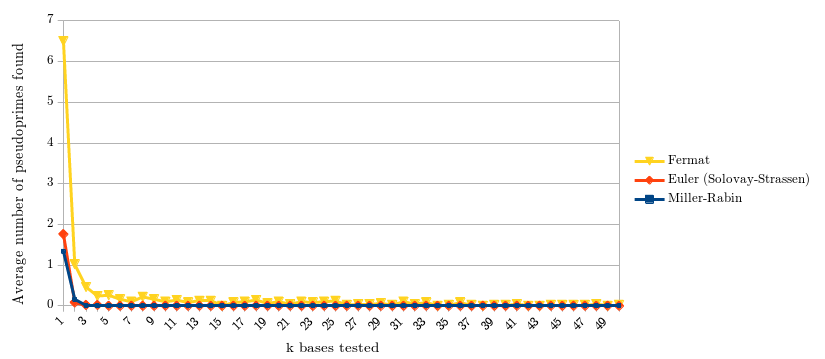
\includegraphics[width=\textwidth]{pprimes_v_bases}
\end{figure}
\FloatBarrier

\FloatBarrier
\begin{figure}[h!]
\caption{Average pseudoprimes passed across all $1 \leq k \leq 50$ values per trial}
\label{fig:pprimes_v_trial}
\centering
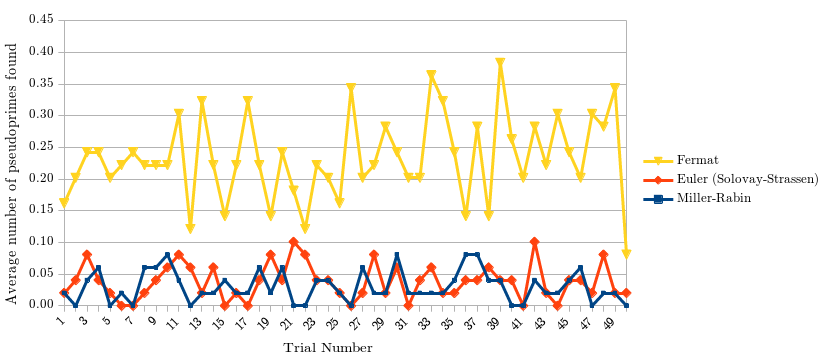
\includegraphics[width=\textwidth]{pprimes_v_trial}
\end{figure}
\FloatBarrier

\FloatBarrier
\begin{figure}[h!]
\caption{The effect of increasing the number of base trials $k$ on running time elapsed}
\label{fig:time_v_bases}
\centering
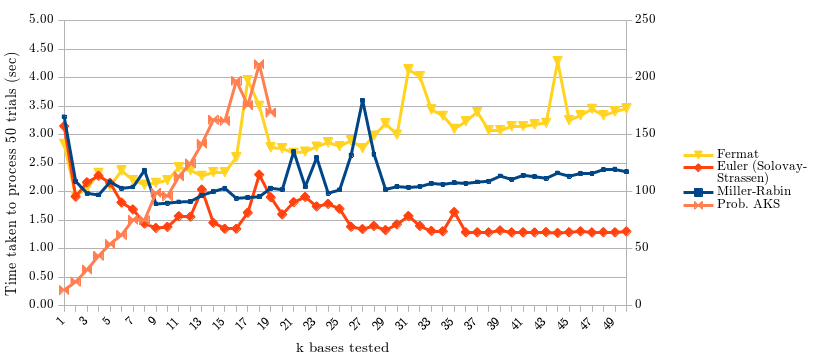
\includegraphics[width=\textwidth]{time_v_bases}
\end{figure}
\FloatBarrier

\FloatBarrier
\begin{figure}[h!]
\caption{Running time elapsed across all $1 \leq k \leq 100$ values per trial}
\label{fig:time_v_trial}
\centering
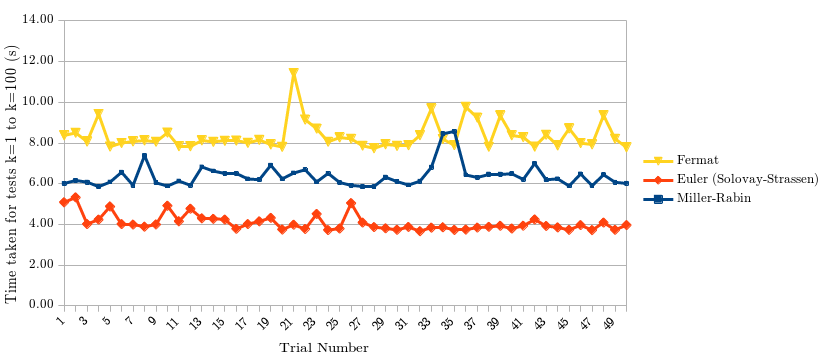
\includegraphics[width=\textwidth]{time_v_trial}
\end{figure}

\FloatBarrier
\begin{figure}[h!]
\caption{Projected average number of pseudoprimes passed by AKS versus other probabilistic tests}
\label{fig:paks_proj_pprimes_v_bases}
\centering
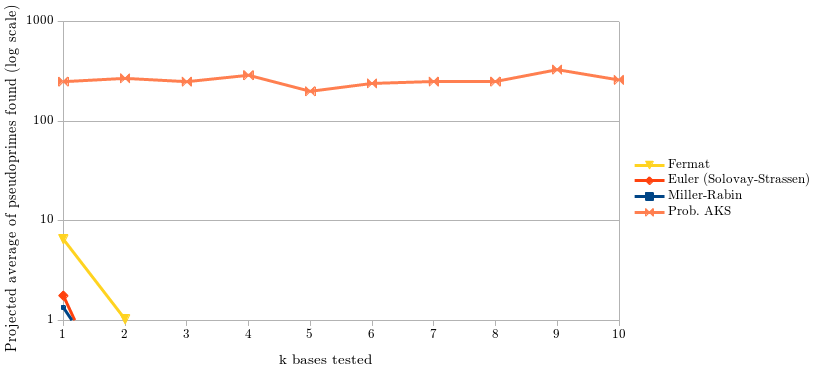
\includegraphics[width=\textwidth]{paks_proj_pprimes_v_bases}
\end{figure}
\FloatBarrier

\FloatBarrier
\begin{longtable}{l|lllllll|l}
\caption{Number of pseudoprimes passed at given $k$ values\label{table:paks_pprimes_v_bases}}\\
\multicolumn{1}{l}{} & \multicolumn{7}{c}{Pseudoprimes passed} &                       \endfirsthead
k-value              & 0 & 1 & 2 & 3 & 4 & 5 & 6               & Average pseudoprimes  \\
\midrule
100                  & 0 & 1 & 2 & 1 & 3 & 0 & 2               & 3.4                   \\
200                  & 1 & 0 & 4 & 0 & 3 & 0 & 0               & 2.6                   \\
300                  & 3 & 0 & 4 & 1 & 1 & 0 & 0               & 1.7                   \\
400                  & 4 & 0 & 4 & 2 & 0 & 0 & 0               & 1.4                   \\
\bottomrule
\end{longtable}
\FloatBarrier

\pagebreak
\FloatBarrier
\begin{figure}[h!]
\caption{Elapsed running time for probabilistic versus deterministic AKS}
\label{fig:paks_v_daks}
\centering
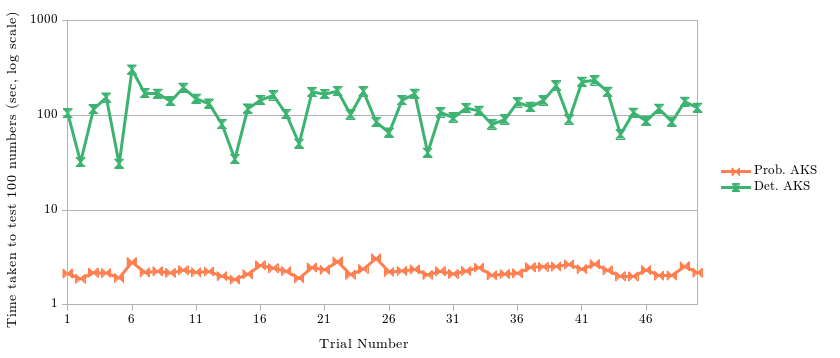
\includegraphics[width=\textwidth]{paks_v_daks}
\end{figure}
\FloatBarrier

\FloatBarrier
\begin{figure}[h!]
\caption{Distribution of pseudoprimes found between $10^5$ and $10^6$ for probabilistic primality tests}
\label{fig:pprimes_passed}
\centering
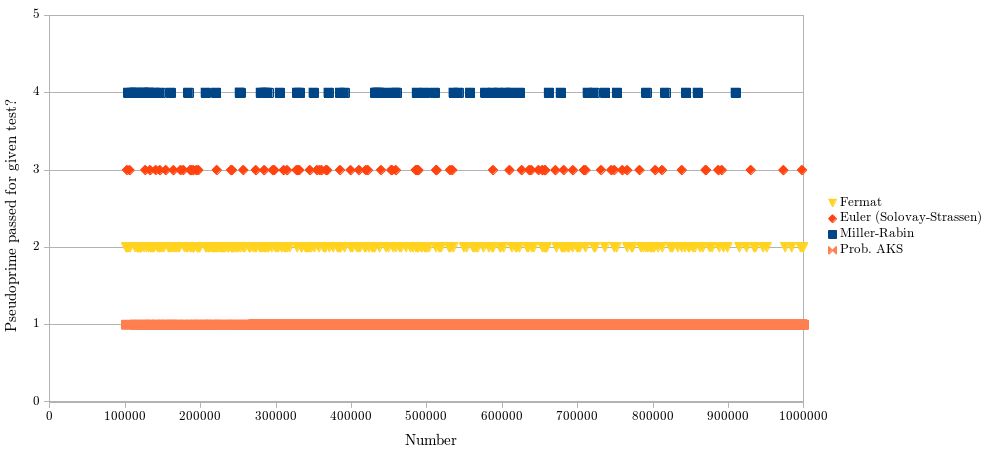
\includegraphics[width=\textwidth]{pprimes_passed}
\end{figure}
\FloatBarrier

\section{Discussion}
Figures \ref{fig:pprimes_v_bases} through \ref{fig:time_v_trial} show various aspects of performance for the Fermat, Euler (Solovay-Strassen), and Miller-Rabin primality tests. From Figures \ref{fig:pprimes_v_bases} and \ref{fig:pprimes_v_trial}, it is clear that the Fermat primality test consistently passes more pseudoprimes compared to the other tests regardless of $k$, as well as having the highest initial average of pseudoprimes passed. As well, the performances of the Euler and Miller-Rabin tests appear nearly identical, though Figure \ref{fig:pprimes_v_trial} reveals the Miller-Rabin test slightly outperforms the Euler test on average. This is supported by the general results demonstrated by Pomerance, Selfridge, and Wagstaff in their 1980 analysis on pseudoprimes to $25 \times 10^9$ \cite{pomerance_pseudoprimes_1980}. There, they found there are 167 Fermat pseudoprimes, 78 Euler pseudoprimes, and 30 strong (Miller-Rabin) pseudoprimes between $10^5$ and $10^6$, indicating the order of increasing performance, in terms of minimizing pseudoprimes passed, is Fermat, Euler, and Miller-Rabin. The Euler and Miller-Rabin results are also supported by other previous research: in 1978, Monier proved the accuracy of the Miller-Rabin primality test was about twice that of the Euler test \cite{monier_evaluation_1980}. While the rate of passed pseudoprimes found in this analysis was not as high, the results shown here (in Figure \ref{fig:pprimes_passed} especially) clearly depict an increase in accuracy.

However, in terms of elapsed running time, the Euler (Solovay-Strassen) test succeeds best, as shown in Figures \ref{fig:time_v_bases} and \ref{fig:time_v_trial}. Where the Fermat and Miller-Rabin tests both increase in time elapsed as increasing numbers of $k$ bases are tested, the Euler test decreases in time until around $k = 35$, before becoming relatively stable with an average runtime lower than all other tests. The findings for the Fermat, Euler, and Miller-Rabin tests contrast the theoretical runtime complexity of each of these algorithms. With a theoretical runtime of $O(k \times \log{n})$, the Fermat test was expected to be the fastest. As well, the theoretical complexity of both the Euler and Miller-Rabin tests is $O(k \times \log^3{n})$, indicating they should theoretically have run in about the same time. The contradictory results shown in this paper may illustrate the difference between theoretical and empirical results, however. A possible explanation for the more efficient runtime of the Euler and Miller-Rabin tests may be the speed at which the algorithms disqualify a number as a prime. As each primality test checks for different properties of prime numbers, the congruences used in the Euler and Miller-Rabin tests may more quickly determine if a number is composite and exit the program, reducing overall time spent on additional calculations. The same hypothesis may apply for the discrepancies in the Euler and Miller-Rabin test performances. The significant increase in time elapsed as $k$ increases for probabilistic AKS is as expected, especially when compared to the results for the other primality tests. As the probabilistic AKS algorithm has a projected worst-case runtime of $\widetilde{O}(k \times \log^5{n})$ compared to the Euler and Miller-Rabin bound of $O(k \times \log^3{n})$, the larger slope of the probabilistic AKS trend supports the complexity proposed.

The next several figures show the performance of probabilistic AKS against other primality tests. Figure \ref{fig:paks_proj_pprimes_v_bases} indicates that probabilistic AKS returns significantly more (around 200) pseudoprimes compared to the other tests. Note the use of a logarithmic scale as well - the accuracy of probabilistic AKS appears extremely low. This is likely due to the relatively low $k$ values of equations tested in probabilistic AKS. While the deterministic AKS algorithm was originally designed to check $\lfloor \sqrt{\phi(r)}\log(n) \rfloor$ bases, the analysis here only shows average projected values for $1 \leq k \leq 10$. Within the bounds of numbers tested, the value of $\lfloor \sqrt{\phi(r)}\log(n) \rfloor$ is around 400 to 500, meaning such low $k$ values were extremely unlikely to return accurate results.

This is supported by data shown in table \ref{table:paks_pprimes_v_bases}, which indicates the number of pseudoprimes returned over 10 trials of $k = 100, 200, 300, 400$. As shown by the table, the distribution of numbers of pseudoprimes passed decreases significantly as $k$ grows larger, from an average of 3.6 pseudoprimes per $10^2$ tests at $k = 100$ to 1.4 at $k=400$. This was as expected, as when $k$ tends towards the value of $\lfloor \sqrt{\phi(r)}\log(n) \rfloor$, the accuracy of probabilistic AKS grows closer to the performance of deterministic AKS. This implies for similar performance to the Fermat, Euler (Solovay-Strassen), and Miller-Rabin tests, a range of $k$ values close, but not equal to, the maximum $\lfloor \sqrt{\phi(r)}\log(n) \rfloor$ should be tested. As supported by the analysis done for this paper, a $k$ range of around 90\% of this value may provide maximum performance, though this is yet to be theoretically verified.

Though deterministic AKS is theoretically proven and guaranteed to produce no pseudoprimes, its runtime is much too slow for practical applications. Rotella's 2005 thesis on efficiently implementing the deterministic AKS algorithm showed times of about 60 to 100sec for determining the primality of a number between 7000 and 8000 \cite{rotella_efficient_2005}. The deterministic AKS implementation used in this paper is faster than the one demonstrated in Rotella's paper, but the trends shown in Figure \ref{fig:paks_v_daks} still highlight the relative inefficiency of the algorithm. (Again, note the use of a logarithmic scale.) The probabilistic AKS algorithm consistently runs in significantly faster time than deterministic AKS, and has less exaggerated variance in performance (perhaps due to a fewer equations checked that disqualify a number from being prime) Though $k=1$ is used to determine speed, the speed improvements remain notable even with higher $k$ values, like $k=20$.

For a visual representation of the distribution of the pseudoprimes passed by each of the tests, see Figure \ref{fig:pprimes_passed}. These results again contrast with the findings of Pomerance et al., as the analysis shown presents far greater numbers of pseudoprimes than in their research \cite{pomerance_pseudoprimes_1980}. This may be due to the fact that a value of $k=1$ was used for the generation of this figure for all primality tests, whereas the table created by Pomerance et al. may have considered larger numbers of bases, or even all bases less than the tested number. Nevertheless, this again supports the accuracy analysis of the four probabilistic primality tests shown here: probabilistic AKS returns the greatest number of pseudoprimes, followed by the Fermat, Euler, and Miller-Rabin primality tests in that order. 

These results show that probabilistic AKS lies between the established probabilistic primality tests and deterministic AKS in terms of identifying minimal pseudoprimes and running with satisfactory speed, supporting the hypotheses identified in Section \ref{paks}. As well, the expected increase in speed was observed, empirically supporting the proposed lowered worst-case runtime complexity of $O(\log^5{n})$. While the probabilistic AKS test is both slower and less accurate at low $k$ values than the three existing probabilistic tests analyzed, it remains a viable option to combine the methodology of the AKS algorithm with acceptable speed and performance for applied usage.

Overall, the Fermat primality test, though simple to implement, is both less accurate and slower than the Euler and Miller-Rabin tests. Therefore, if wishing to optimize for speed, the Euler test may be recommended, and if a lower probability of passing pseudoprimes is desired, the Miller-Rabin test is a practical alternative. If complete accuracy and determinism is of importance, the deterministic AKS test is the best choice out of the primality tests discussed in this paper. However, if determinism can be sacrificed for an improvement in theoretical and practical runtime in situations where deterministic AKS would otherwise be used, the probabilistic AKS variant may be an adequate option.

\section{Sources of Error}
\label{soe}
A possible source of error present includes the range of numbers tested for pseudoprimes and the distribution of pseudoprimes over said range. Again, as Pomerance et al. showed, there are 167 Fermat pseudoprimes, 78 Euler (Solovay-Strassen) pseudoprimes, and 30 Miller-Rabin pseudoprimes in the interval tested in this paper ($10^5 \leq x \leq 10^6$) \cite{pomerance_pseudoprimes_1980}. These values increase for higher numbers, and it is possible that the bounds examined in this paper were insufficient to reveal unexpected behaviour that may occur with different bounds.

Another potential source of error was the $k$ value analysis for the probabilistic AKS test. Due to time constraints, only certain $k$ values were tested, with smaller numbers of random integers tested with each trial ($10^2$ instead of $10^4$). These $k$ values were not consistent with the ones tested in the Fermat, Euler, and Miller-Rabin trials, which may not allow for standardized comparisons. For example, in Figure \ref{fig:paks_proj_pprimes_v_bases}, the average number of pseudoprimes is projected, instead of experimentally measured. This may have led to inaccuracies in comparisons and analysis. Due to time constraints, the number of trials conducted for probabilistic AKS also differed (10 vs. 50), which may lead to outlier trials overly affecting the averages for the probabilistic AKS trials.

A last possible source of error was the primality test used to verify each test, the inbuilt \texttt{isprime} function in Sympy. As the function uses a variant of the Baillie-Pomerance-Selfridge-Wagstaff test, which is itself probabilistic, there is a possibility additional pseudoprimes were passed but not detected by either the \texttt{isprime} function or the primality tests.

\section{Further Research}
As mentioned in section \ref{soe}, the distribution of pseudoprimes for each of the tests varies with the upper and lower bounds chosen. In larger intervals between larger numbers, the amount of these pseudoprimes grows. However, with larger intervals, the probability of randomly selecting pseudoprimes within $10^4$ choices decreases. Increasing the bounds of the tests was outside the scope of this examination, but may be left to future research. 

As well, the $k$ values in data collected for the probabilistic AKS test were not identical to those analyzed for the Fermat, Euler, and Miller-Rabin tests. With values of $1 \leq k \leq 50$, however, it was unlikely reasonable analysis could be done, as the number of equations tested was too low to give any meaningful results. In the future, finding the approximate range of $k$ where the number of pseudoprimes found begins to range similarly to the values found at $1 \leq k \leq 50$ for the other probabilistic tests may allow closer comparison between the tests. As well, running additional trials (50 total) for each of the $k$ values for the probabilistic AKS test will allow for a larger overview of the test's performance to be formed.

To rectify the final source of error discussed in section \ref{soe}, an alternative primality test may be used to verify the primality instead of the Sympy \texttt{isprime} function. For example, though deterministic AKS is impractical to repeatedly test with large numbers of integers, given enough time and computing power, a deterministic index of all integers in the testing interval may be built. This would allow for a direct comparison with a deterministically verified primes list, and eliminate the chance for missing any pseudoprimes in analysis.

In the future, looking deeper into potential bound refinements for deterministic and probabilistic AKS may also improve the algorithms and their theoretical running time. As with the deterministic AKS algorithm, the main limiting factor in increasing the speed of probabilistic AKS is the bounds of $r$, the value used to determine the upper bound for polynomial congruences to check. A possible further optimization for AKS in general is detailed in Nemana and Venkaiah's empirical study on reducing the number of polynomial equivalences to compute \cite{nemana_empirical_2016}. The paper proposes to find an $r$ such that $(\lceil \log{n} \rceil - 1)^2 \leq r \leq 2 \times (\lceil \log{n} \rceil)^2$, $r$ is prime, and $\textrm{ord}_r(n) \geq \lfloor \log^2{n} \rfloor$. This would reduce the time complexity of steps 2, 3, and 5 in the deterministic AKS algorithm, and the modifications can also be applied to probabilistic AKS to further optimize the theoretical runtime bounds. Future analysis, perhaps comparing this variant to the probabilistic variant proposed in this paper and to deterministic AKS, may lead to possible improvements in both probabilistic and deterministic AKS.

\section{Conclusion}
Primality testing is a key building block of modern cryptography, and as such, the study of efficient methods of generating and verifying prime numbers is of interest in contemporary computer science and mathematics. Several well-studied primality tests include the Fermat, Euler (Solovay-Strassen), and Miller-Rabin primality tests, all of which are probabilistic, or include some element of randomness and a small probability that a composite number will be labelled as prime. Other primality tests, known as deterministic primality tests, have been developed that eliminate this chance of passing so-called pseudoprimes. Of these deterministic tests, the Agarwal-Kayal-Saxena test is notable for running in polynomial-bounded time. This paper aimed to discuss these primality tests, comparing the three existing probabilistic tests, and proposing and analyzing a probabilistic variant of AKS.

It was found that while all tests followed similar trends of rapidly decreasing average number of pseudoprimes passed at higher numbers of bases tested $k$ and of increasing running time elapsed with an increasing $k$, different tests were most performant with respect to different variables. The Miller-Rabin test was consistently the most accurate, passing the lowest average number of pseudoprimes at all $k$ values. However, the Euler (Solovay-Strassen) test appeared to unexpectedly decrease in elapsed time with increasing $k$ values, and was most efficient with regards to time. The Fermat test consistently returned more pseudoprimes and was less efficient than either of the Euler or Miller-Rabin tests. While probabilistic AKS returned the most pseudoprimes at low $k$ values ($1 \leq k \leq 50$) compared to the existing probabilistic tests, it offered a ~55x speed increase over deterministic AKS and performed relatively well at higher $k$ values. It does not yet come close to existing probabilistic tests in speed or accuracy at low $k$ values.

Several sources of error were identified, such as potentially overly tight bounds, $k$ value analysis, average number of pseudoprime projection, and the use of probabilistic pseudoprime verification methods. These were addressed in recommendations for future areas of research, including increasing bounds, running additional trials, covering higher values of $k$, and conducting further research on optimizing the bounds of $r$ with probabilistic AKS.

This paper was written under the supervision of Ms. Pressiana Marinova (Ocado Technology Sofia) at the Summer Research School 2021, hosted by the High School Student Institute of Mathematics and Informatics. Many thanks to Ms. Marinova for her exceptional mentorship and thorough guidance, and to HSSIMI for providing a welcoming research environment.

\newpage
\nocite{*}
\bibliographystyle{plainnat}
\bibliography{references}

\appendix
\begin{appendices}
\section{Raw Data for Primality Tests} \label{appendix:data}

The raw data for each of the primality tests can be found \href{https://github.com/kewbish/srs/tree/master/dataset}{here}.
The data is available in CSV format, labelled by primality test (Fermat, Euler, Miller-Rabin, deterministic AKS, and probabilistic AKS). The folder also includes other data not discussed in-depth in this paper, including several base analysis types (all bases generated randomly, base 2, base 3, base 5, or a combination of bases 2 and 3, bases 3 and 5, and bases 2 and 3).

For the majority of the dataset, each row in the CSV file is a trial of the given test with given base. The first hundred columns represent the pseudoprimes found at $k$ trials of different bases. The last four columns represent the average pseudoprimes found over the entire trial from $1 \leq k \leq 100$, the lowest $k$ value required to pass the lowest number of pseudoprimes, the lowest number of pseudoprimes, and the time required to run the test in minutes and seconds. 
The last row, which contains only 50 values, should be interpreted as the average time taken for a trial of $k$ bases, where $k$ is the column number.

The file $\texttt{passed\_pprimes.csv}$ is formatted in a similar method. However, it should be interpreted as lists of all the pseudoprimes passed per test between $10^5$ and $10^6$. The corresponding test is indicated in the first column. Rows 1 through 13 all contain data for probabilistic AKS, split up into rows of 1023 data points to allow for common column limits in spreadsheet software.

The file $\texttt{paks\_arb.csv}$ contains data for all $k$ trials for probabilistic AKS. The first four blocks in rows 1 through 44 contain information for the $k$ value, number of pseudoprimes passed, and time elapsed in seconds for $10^2$ random integers. Rows 45 through 54 contains data for ten trials of probabilistic with $1 \leq k \leq 10$, with averages and elapsed time in seconds at the end of each row. Row 55 contains the average number of pseudoprimes for each $k$ value. Row 57 contains the average elapsed time in seconds required for probabilistic AKS with $1 \leq k \leq 20$.

The file $\texttt{paks\_v\_daks.csv}$ contains the timing data for 50 trials of probabilistic and deterministic AKS over $10^2$ integers. The first row is the elapsed time in seconds for probabilistic AKS; the second row provides the data points for deterministic AKS.

\section{Technical Details} \label{appendix:tech}

\subsection{Primality Test Implementations}
The implementations of the primality tests can be found on GitHub at \href{https://github.com/kewbish/srs}{kewbish/srs}.
The tests were implemented with Python 3.9.6, with the \href{https://numpy.org/}{Numpy} and \href{http://numba.pydata.org/}{Numba} libraries used to optimize computations, and the \href{Sympy}{https://www.sympy.org/en/index.html} library used to test for primality.
The AKS primality test implementation was improved on from a reference implementation by Sophoclis Stephanou found on GitHub \cite{stephanou_ssophoclis/aks-algorithm:_2020}.

\subsection{Hardware}
The primality tests ran on a HP-15bs028ca running Manjaro Linux x86\_64 and kernel 5.10.49-1-MANJARO, with a 4-core Intel i5-7200U 3.100GHz CPU and 16.0GiB of RAM.

\end{appendices}

\end{document}

